\documentclass{article}

\usepackage[spanish]{babel}
\usepackage[utf8]{inputenc}
\usepackage{graphicx}
\graphicspath{{images/}}

\title{Trabajo Practico 1: Unidad Aritmética Lógica}
\author{Perez, Federico\\
        \texttt{perezfederico@unc.edu.ar}
        \and 
        Sardoy, Juan Manuel\\
        \texttt{jmsardoy@gmail.com}
        }
\begin{document}
\maketitle
\\
\begin{center}
    
\includegraphics[scale=2]{unc-logo}
\end{center}
\newpage
\section{Descripción del trabajo}

Se trata de la implementación de una unidad aritmética lógica (ALU) en FPGA
utilizando el lenguaje de descripción de hardware verilog.\\
\indent La ALU deberá poder realizar las operaciones listadas a continuación, y
deberá reconocer cada una de ella según el código que se ingrese:\\ 

\begin{center}
    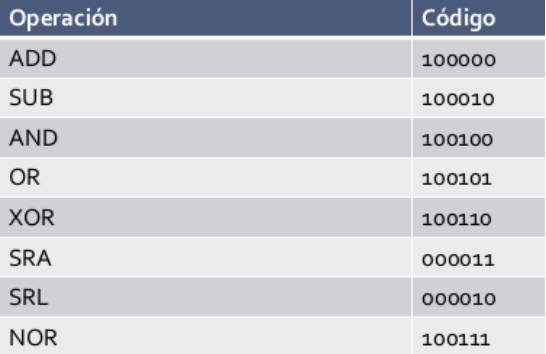
\includegraphics[scale=0.5]{opcodes}
\end{center}

\indent La ALU recibirña dos valores como entradas (A y B) y un tercer valor
que será el opcode de la operación a realizar. Estos valores ingresarán por
medio de los switchs de la placa Basys 2, y sus pulsadores, uno por cada input.
El resultado luego se verá en binario en los LEDs de la placa.\\
\indent La ALU deberá ser parametrizable respecto del ancho de bus (por defecto
resuelve operaciones con valores de 8 bits).

\section{Implementación}
El trabajo se divide en dos modulos: ALU y Top\_level.\\
\indent El módulo ALU es la unidad aritmética lógica, y solo se encarga de
resolver cual es la operación dada por el opcode mediante una sentencia case, y
luego resolverla combinacionalmente.\\
\indent El módulo Top\_level se encarga de instanciar el módulo ALU y recibir
los valores A, B y el opcode desde los pulsadores correspondientes.

\section{Simulación}
Para corroborar el buen funcionamiento del módulo ALU, se realizo una
simulación por software del mismo.\\
\indent El resultado de la simulación fue:
\begin{center}
    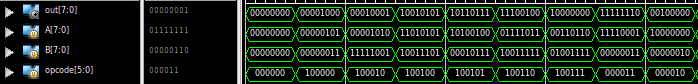
\includegraphics[scale=0.55]{simulacion}
\end{center}
\indent Se probaron todas las operaciones comprobando sus resultados.
\end{document}
